\documentclass{article}
\usepackage{graphicx}
\usepackage{float}
\title{Crowbar Test with Subtracted Reference}
\author{MiKaela Barker}

\begin{document}

\maketitle
Measurements taken have a subtracted reference made by averaging several references. These references are formed from the average of four rotation angles of the MOSES I primary mirror. Experimentation completed June 16, 2017, for MOSES III instrumentation testing. Measurements shown are an average of 32 single interferogram measurements using 4Sight software. Zernike values are taken from the in-program Zernike polynomial worksheet. For use in comparing placement of the mirror to overall mirror surface aberrations, in order to prepare to correct mirror figure. Definitions for each of the tests can be found in Section \ref{descriptors}. 

\section{Graph of Individual Tests}
The first ten Zernike polinomials are taken from the 4Sight software and used to generate visual graphs to determine the ideal positioning of the MOSES II mirror in its flight mount. The following are several graphs showing this. The first shows all tests and all polinomials. The following are individual tests.

\begin{figure}[h!]
	\centering
	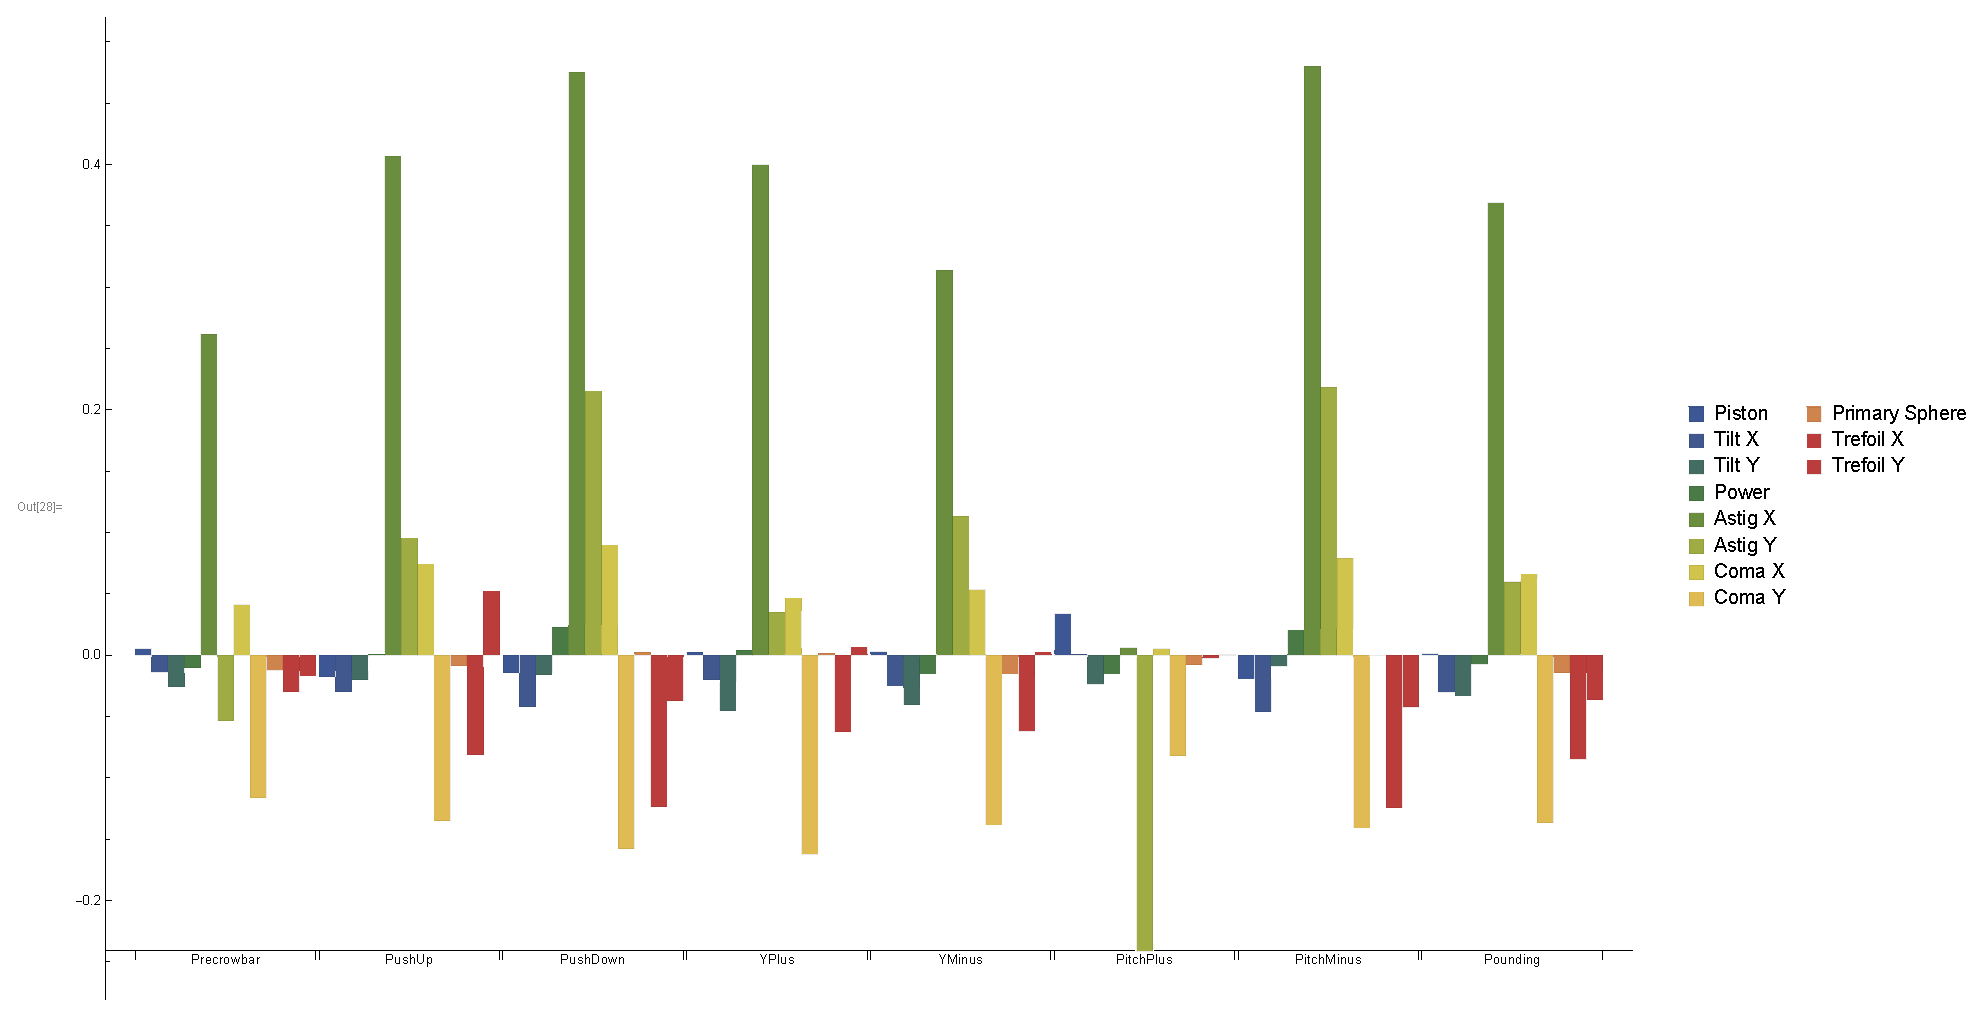
\includegraphics[width=.8\linewidth]{GraphData_IndividualTests_minusref2.eps}
	\caption{Chart of All Test Zernikes}
	\label{minrefgraph}
\end{figure}
\begin{figure}
	\centering
	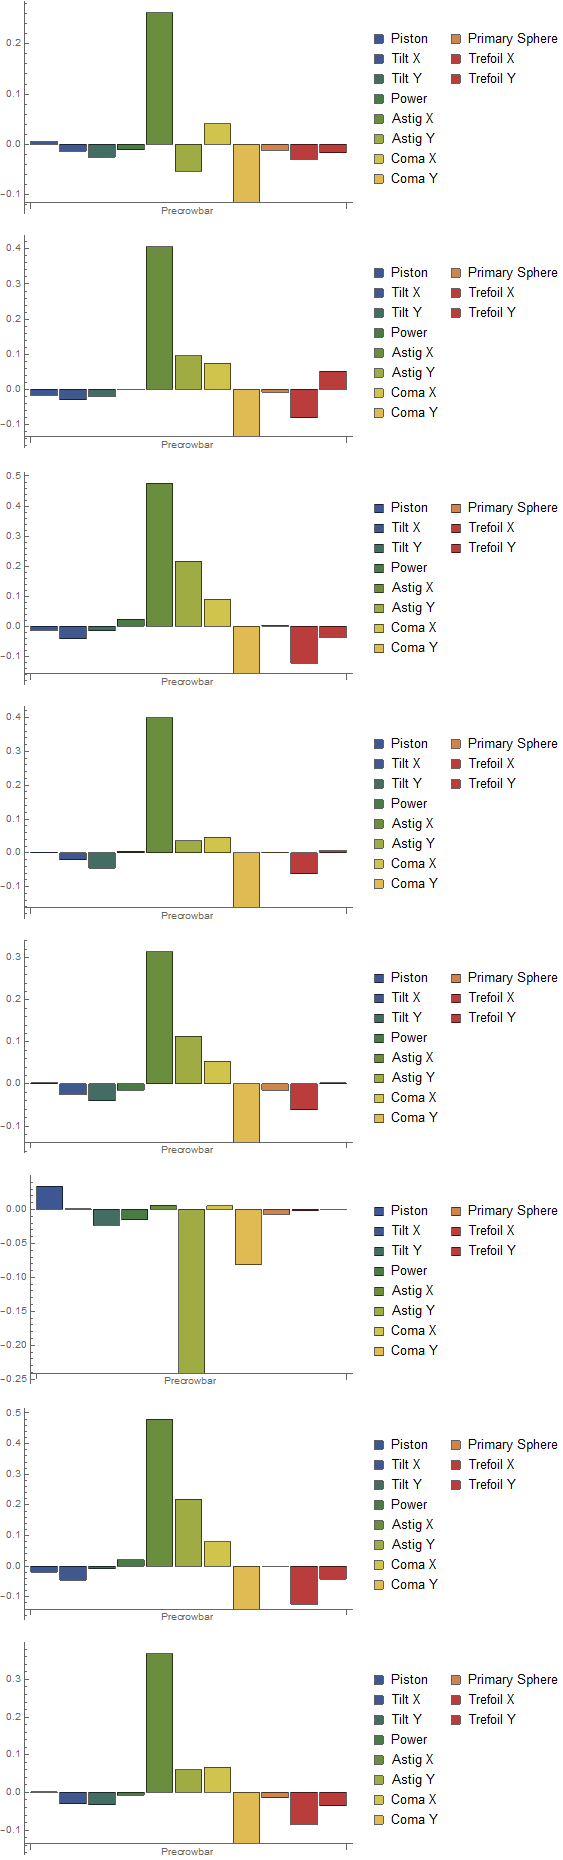
\includegraphics[scale=0.25]{GraphData_IndividualTests_minusref2}
	\caption{*LabelinngSystem*}
	\label{alltestsminref}
\end{figure}

\section{Zernike Values}
\begin{table}[H]
	\centering
	\begin{tabular}{r|p{1in}} \hline
		Piston &0.0055 \\
		Tilt X &-0.0135\\
		Tilt Y &-0.0255\\
		Power &-0.0102\\
		Astig X &0.26193\\
		Astig Y &-0.0531\\
		Coma X &0.0412\\
		Coma Y &-0.11578\\
		Primary Sphere &-0.0119\\
		Trefoil X &-0.0295\\
		Trefoil Y &-0.0168
	\end{tabular}
	\caption{Pre-crowbar Zernikes}
	\label{precrowbar}
\end{table}
\begin{table}[H]
	\centering
	\begin{tabular}{r|p{1in}} \hline
		Piston &-0.0172 \\
		Tilt X &-0.0295\\
		Tilt Y &-0.0199\\
		Power &0.0068\\
		Astig X &0.4065\\
		Astig Y &0.0958\\
		Coma X &0.0744\\
		Coma Y &-0.1344\\
		Primary Sphere &-0.0083\\
		Trefoil X &-0.0806\\
		Trefoil Y &0.0524
	\end{tabular}
	\caption{Push-Up Zernikes}
	\label{pushup}
\end{table}
\begin{table}[H]
	\centering
	\begin{tabular}{r|p{1in}} \hline
		Piston &-0.0140 \\
		Tilt X &-0.0417\\
		Tilt Y &-0.0157\\
		Power & 0.0228\\
		Astig X & 0.47535\\
		Astig Y & 0.21550\\
		Coma X & 0.0902\\
		Coma Y &-0.15770\\
		Primary Sphere &0.0023\\
		Trefoil X &-0.12311\\
		Trefoil Y &-0.0369
	\end{tabular}
	\caption{Push-Down Zernikes}
	\label{pushdown}
\end{table}
\begin{table}[H]
	\centering
	\begin{tabular}{r|p{1in}} \hline
		Piston &0.0023 \\
		Tilt X &-0.0198\\
		Tilt Y &-0.0449\\
		Power & 0.0042\\
		Astig X & 0.4000\\
		Astig Y & 0.0352\\
		Coma X &0.0469\\
		Coma Y &-0.1621\\
		Primary Sphere &0.0017\\
		Trefoil X &-0.0621\\
		Trefoil Y & 0.0069
	\end{tabular}
	\caption{Plus-Y Zernikes}
	\label{yplus}
\end{table}
\begin{table}[H]
	\centering
	\begin{tabular}{r|p{1in}} \hline
		Piston &0.0030\\
		Tilt X &-0.0249\\
		Tilt Y &-0.0402\\
		Power &-0.0151\\
		Astig X &0.31394\\
		Astig Y &0.11321\\
		Coma X &0.0535\\
		Coma Y &-0.13815\\
		Primary Sphere &-0.0151\\
		Trefoil X &-0.0618\\
		Trefoil Y &0.0027
	\end{tabular}
	\caption{Minus-Y Zernikes}
	\label{yminus}
\end{table}
\begin{table}[H]
	\centering
	\begin{tabular}{r|p{1in}} \hline
		Piston &0.0340\\
		Tilt X &0.0008\\
		Tilt Y &-0.0233\\
		Power &-0.0150\\
		Astig X &0.0063\\
		Astig Y &-0.24092\\
		Coma X &0.0056\\
		Coma Y &-0.0815\\
		Primary Sphere &-0.0073\\
		Trefoil X &-0.0021\\
		Trefoil Y &0.0003
	\end{tabular}
	\caption{Pitch-Plus Zernikes}
	\label{pitchplus}
\end{table}
\begin{table}[H]
	\centering
	\begin{tabular}{r|p{1in}} \hline
		Piston &-0.0194\\
		Tilt X &-0.0457\\
		Tilt Y &-0.0090\\
		Power &0.0206\\
		Astig X &0.48005\\
		Astig Y &0.21838\\
		Coma X &0.0794\\
		Coma Y &-0.14061\\
		Primary Sphere &-0.00006397\\
		Trefoil X &-0.12392\\
		Trefoil Y &-0.0420
	\end{tabular}
	\caption{Pitch-Minus Zernikes}
	\label{pitchminus}
\end{table}
\begin{table}[H]
	\centering
	\begin{tabular}{r|p{1in}} \hline
		Piston &0.0013\\
		Tilt X &-0.0301\\
		Tilt Y &-0.0329\\
		Power &-0.0072\\
		Astig X &0.36879\\
		Astig Y &0.0599\\
		Coma X &0.0664\\
		Coma Y &-0.13620\\
		Primary Sphere &-0.0138\\
		Trefoil X &-0.0846\\
		Trefoil Y &-0.0358
	\end{tabular}
	\caption{Pounding Zernikes}
	\label{pound}
\end{table}

\section{Test Name Descriptions}\label{descriptors}
Pre-Crowbar displayes the measuremnts of the mirror before any adjustments were made. Pitch Plus shows a movement of the mirror such that it is tilted in the plus direction. Pitch Minus is the opposite---the mirror is tilted in the minus direction. Push Up is a shift of the mirror upwards from center in the mount. Push Down, a shift of the mirror downwards from center in the mount. Push  Y Plus is a shift of the mirror in the Y+ direction according to MOSES coordinates. Push Y Minus is a shift in the mirror in the Y- direction in the mirror mount. Pounding is the shifting of the mirror in various directions with the purpose to settle it into a position of least tension, and therefore, lowest energy.

\end{document}
